\chapter{Transformer} \label{chap:transformer}

We already have a glimpse of the architecture of transformers in Section \ref{sec:transformer_overview}. In this chapter, we will introduce the remaining components of transformer blocks. Figure \ref{fig:encoder_decoder} gives a close look into a transformer block.

\begin{figure}
    \centering
    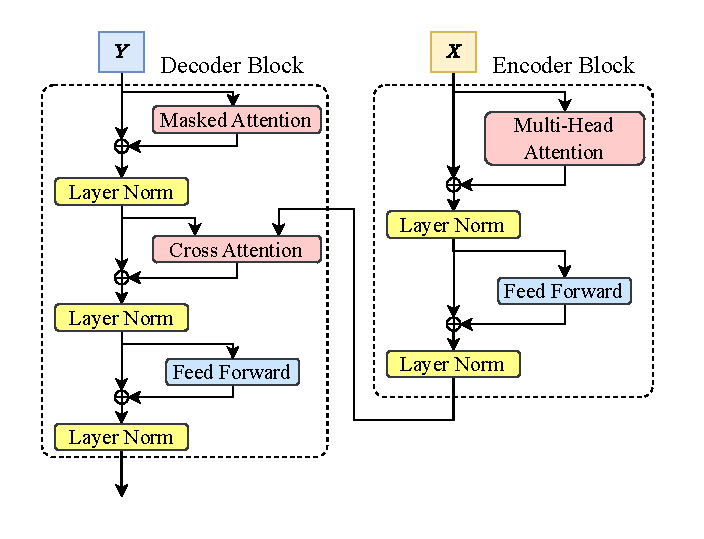
\includegraphics[width=0.8\linewidth]{fig/encoder_decoder.pdf}
    \caption{Transformer blocks. More specifically, they are an encoder block and a decoder block, which are explained in Section \ref{sec:encoder_decoder}.}
    \label{fig:encoder_decoder}
\end{figure}

% As a quick recap, a transformer consists of embedding layers and transformer blocks, where the latter have four components:

% \begin{itemize}
%     \item \textbf{an attention layer},
%     \item \textbf{a feedforward layer},
%     \item \textbf{normalization layers (layer norms)}, and
%     \item \textbf{residual connections},
% \end{itemize}

\section{Feedforward Layer}

The \textbf{feedforward layer} in transformer blocks is a fully-connected 2-layer neural network with ReLU activation, which can be written as
$$
\text{FFN}(x) = \max(0, xW_1+b_1)W_2 + b_2,
$$
where $W_1 \in \mathbb{R}^{d\times d_{ff}}$ and $W_2 \in \mathbb{R}^{d_{ff}\times d}$. (In the original paper \cite{vaswani2017attention}, the authors chose $d_{ff} = 2048 = 4d$.)
% In practice, the choice of $d_{ff}$ is often approximately $4d$. 
Feedforward layers add non-linearity into the transformer architecture, and extend the information captured by attention mechanism. Note that the weights are shared across inputs, which means that the calculations here are independent among input tokens.

\section{Layer Normalization (Layer Norm)}

In transformer blocks, \textbf{layer normalization} performs normalization on \textit{each input embedding}: Given an input embedding $x = (\chi_1, \cdots, \chi_d)$, layer normalization calculates the following:
\begin{equation}
\begin{aligned}
    \mu &= \sum_{i=1}^d \chi_i, \\
    \sigma &= \sqrt{\frac{1}{d}\sum_{i=1}^d(\chi_i - \mu)^2}, \\
    \chi_i &\leftarrow \gamma_i\frac{\chi_i - \mu}{\sigma} + \beta_i,
\end{aligned}
\end{equation}
where $\gamma$ and $\beta$ are parameters. Normalization is adopted to improve training performance, say, prevent gradient underflow/overflow. Note that the normalization process is performed \textit{feature-wise}, but not on the whole input sequence. This ensures that each feature (input embedding) remains its independence in terms of the information it captures. Finally, trainable parameters $\gamma = (\gamma_1, \cdots, \gamma_d)$ and $\beta = (\beta_1, \cdots, \beta_d)$ are introduced to restore the representational capacity of normalized embeddings, by learning a suitable scale and shift for each feature (i.e., each of the $d$ dimensions).

\section{Residual Connection}

A \textbf{residual connection} is a shortcut connection added to a neural network that bypasses one or more layers, which eases the problem of gradient vanishing. For example, consider a 2-layer feedforward network $\mathcal{N}$: $L_1(x) = xW_1 + b_2, L_2(x) = xW_2 + b_2$, and the output of this network is $y = L_2(L_1(x))$. Adding residual connection transforms the output into $y_{res} = L_2(L_1(x)) + L_1(x)$. To see why gradients might vanish, consider the following equations:
\begin{align*}
  \frac{\partial y}{\partial W_1} &= \frac {\partial y}{\partial L_2} \frac {\partial L_2}{\partial L_1} \frac {\partial L_1}{\partial W_1}, \tag{*} \label{eq:3.3.1} \\
  \frac{\partial y_{res}}{\partial W_1} &= \underbrace{\frac {\partial y_{res}}{\partial L_2} \frac {\partial L_2}{\partial L_1} \frac {\partial L_1}{\partial W_1}}_{\text{Vanish!}} + \frac {\partial y_{res}}{\partial L_1} \frac {\partial L_1}{\partial W_1}. \tag{**}\label{eq:3.3.2} \\
\end{align*}    
The original gradient (\ref{eq:3.3.1}) for $\mathcal{N}$ only involves a multiplicative term, which might be extremely small due to continual multiplications. In contrast, the addition of $\frac{\partial y_{res}}{\partial L_1} \frac {\partial L_1}{\partial W_1}$ in (\ref{eq:3.3.2}) from the residual connection is capable of mitigating this issue. The $\oplus$ in Figure \ref{fig:encoder_decoder} indicate residual connections in transformers.

\section{Encoder and Decoder Block} \label{sec:encoder_decoder}

\begin{CJK*}{UTF8}{bkai}
Inside the transformer architecture, there are two types of transformer blocks: encoder and decoder. Take a machine translation task for example. (Recall that transformer was originally proposed for translation in \cite{vaswani2017attention}.) Suppose we would like to translate ``你好嗎?" into English. An \textbf{encoder} is responsible for \textit{encoding} the whole 
sentence ``你好嗎?". A \textbf{decoder} then utilizes the information learned from the encoder, and 
sequentially outputs the translated sentence ``How are you?". Figure \ref{fig:example_translation} demonstrates this process, and Figure \ref{fig:encoder_decoder} shows the respective components of a encoder and a decoder. There are two variants of attention mechanism behind this encoder-decoder architecture: \textbf{masked attention} and \textbf{cross attention}. Details follow.
\end{CJK*}

\begin{figure}
    \centering
    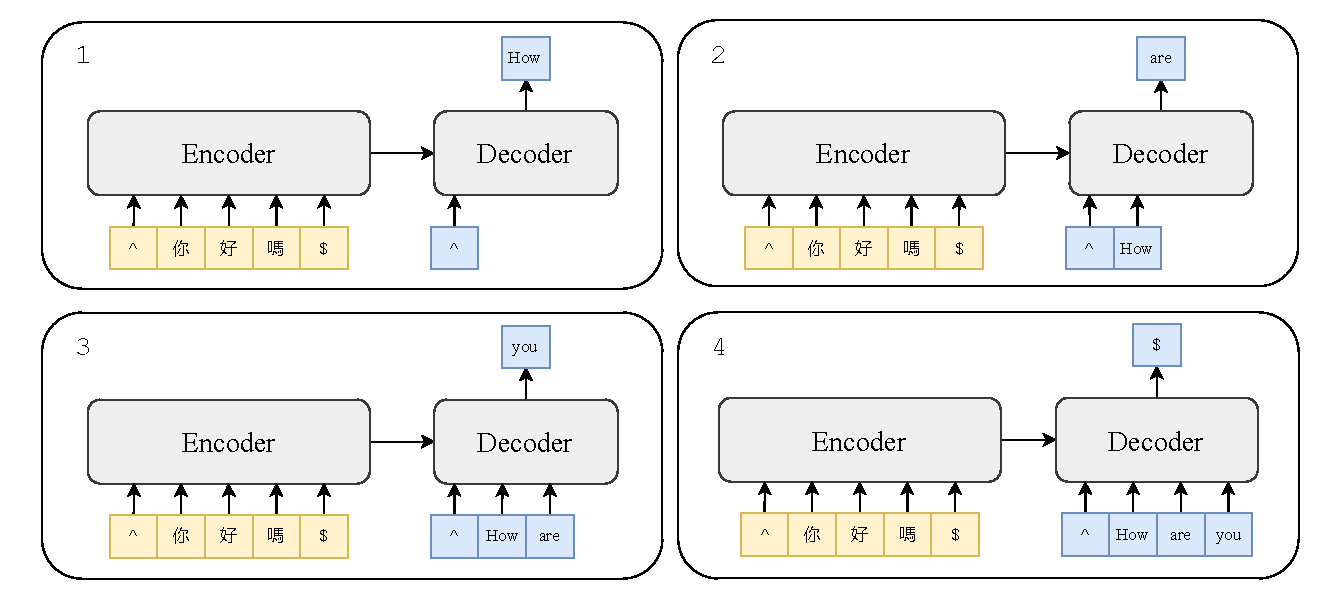
\includegraphics[width=1\linewidth]{fig/example_translation.pdf}
    % \includesvg[width=1\linewidth]{fig/example_translation.svg}
    \caption{Chinese-English translation example, with encoder and decoder blocks.}
    \label{fig:example_translation}
\end{figure}

\subsection{Masked Attention}

Ideally, each input dimension of a decoder should be able to output (predict) the \textit{next} token from its position. If the ordinary attention mechanism is applied (Figure \ref{fig:QK^T}), tokens are able to attend to \textit{future} information, which makes decoding the \textit{next} word trivial! Therefore, in the masked attention mechanism, the upper-triangular portion of $QK^T$ (the \textit{future} information) is ``masked" by $-\infty$, which essentially becomes $0$ after softmax is applied. Figure \ref{fig:masked_attention} illustrates the masked $QK^T$. It is worth mentioning that masking is more relevant to the \textit{training phase} than it would be when transformers are used in production (say, in translating texts) \cite{3b1b}.

\begin{figure}
    \centering
    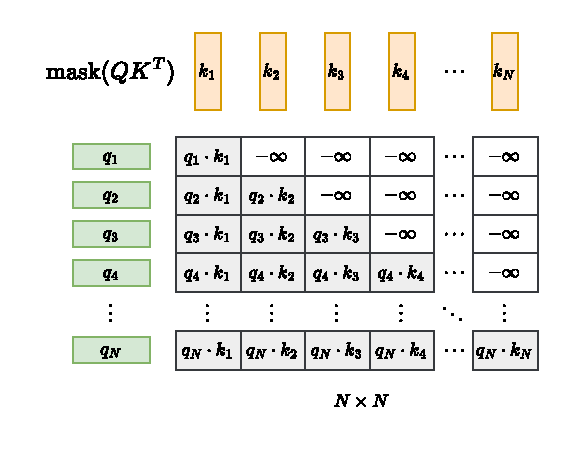
\includegraphics[width=0.8\linewidth]{fig/masked_attention.pdf}
    \caption{Masked attention.}
    \label{fig:masked_attention}
\end{figure}

\subsection{Cross Attention}

How decoders retrieve information from encoders? In the original attention mechanism, all query, key and value come from a single block (e.g. an encoder block). To allow information flows from encoders to decoders, we simply let \textit{decoders query encoders}: The queries $Q$ is from a decoder, and the keys $K$ and values $V$ are from an encoder, as shown in Figure \ref{fig:cross_attention}.

\begin{figure}
    \centering
    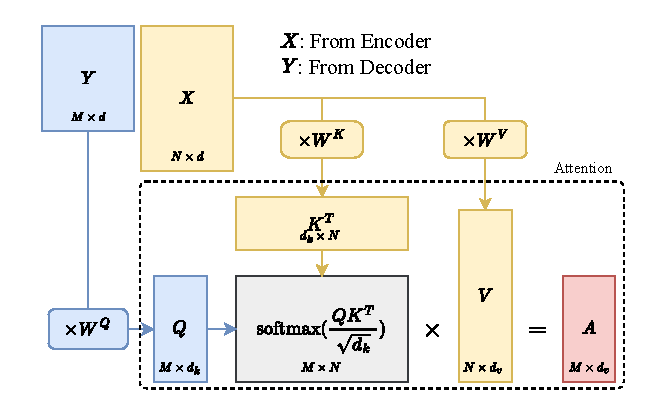
\includegraphics[width=0.8\linewidth]{fig/cross_attention.pdf}
    \caption{Cross attention.}
    \label{fig:cross_attention}
\end{figure}

\section{Embedding Layers}

As briefly sketched in Section \ref{sec:transformer_overview}, embedding layers convert words to vectors and the other way around. We can divide the embedding layers into two categories: \textbf{input embedding layer} and \textbf{output unembedding layer}.

\subsection{Input Embedding Layer}

Each transformer has an input embedding layer, which encodes the following aspects of input words: (1) \textbf{word meanings} (2) \textbf{word positions}. 

For (1), the input word $w$ is first \textbf{one-hot encoded} according to its index in the vocabulary $V$ (i.e., all the words that machines recognize). Suppose $w$ is the $16^{\text{th}}$ word in $V$. Then it would be encoded as $v = (\underbrace{0, \cdots, 0}_{15}, 1, \underbrace{0, \cdots, 0}_{|V|-16})$. Next, the one-hot vector $v$ is multiplied by the $|V|\times d$ \textbf{embedding matrix} $E$, which contains the initial representations for each word in $V$. In practice, $E$ is often pre-trained elsewhere, but not randomly initialized.

For (2), the goal is to encode each possible position of a word in a sequence into some vector of $d$ dimensions. For position $pos$, its encoding $PE(pos)$ is defined as:
\begin{align*}
    PE(pos, 2i) &= sin(pos/10000^{2i/d}), \\
    PE(pos, 2i+1) &= cos(pos/10000^{2i/d}),
\end{align*}
where $0 \le i \le \lfloor d/2 \rfloor$ is the dimension and $10000$ is a pre-defined constant. This encoding is proposed due to the following advantages:

\begin{itemize}
    \item Each position is \textbf{uniquely} encoded, and the model can extrapolate to sequence lengths \textbf{longer} than the ones encountered during training.
    \item It captures \textbf{relative positions} in the following sense: For a fixed offset $k$, $PE(pos + k)$  can be represented as a linear function of $PE(pos)$.
\end{itemize}

To combine (1) and (2), we simply sum them up: The final embedding of $w$ is $e_w := vE + PE(pos_w)$. This layer is summarized in Figure \ref{fig:embedding}.

\begin{figure}
    \centering
    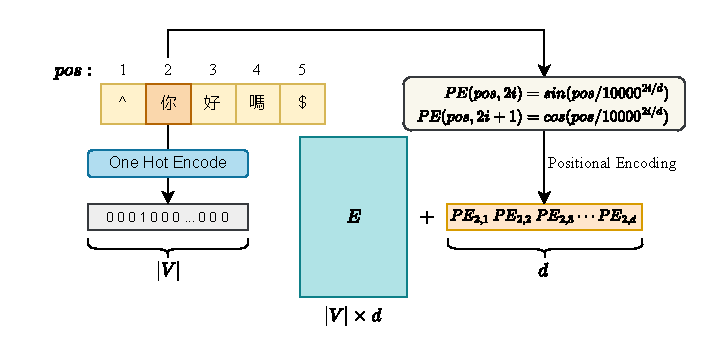
\includegraphics[width=0.9\linewidth]{fig/embedding.pdf}
    \caption{Input embedding layer.}
    \label{fig:embedding}
\end{figure}

\subsection{Output Unembedding Layer}

Each transformer also has an unembedding layer, to map the inner representations of words in a transformer to something we can more easily handle. An \textbf{unembedding matrix} $U$ of size $d \times |V|$ is multiplied to the output $Y$ of the final decoder block to generate the unembedded vectors $Y'$ (called \textit{logits}), i.e., $Y' := YU$. A softmax is then applied to the last row of $Y'$, converting its elements into a probability distribution for further processing (e.g. sampling). In practice, we may choose $U = E^T$, which is the transpose of the \textit{embedding matrix} for parameter-saving. Figure \ref{fig:unembedding} illustrates the whole process.

\begin{figure}
    \centering
    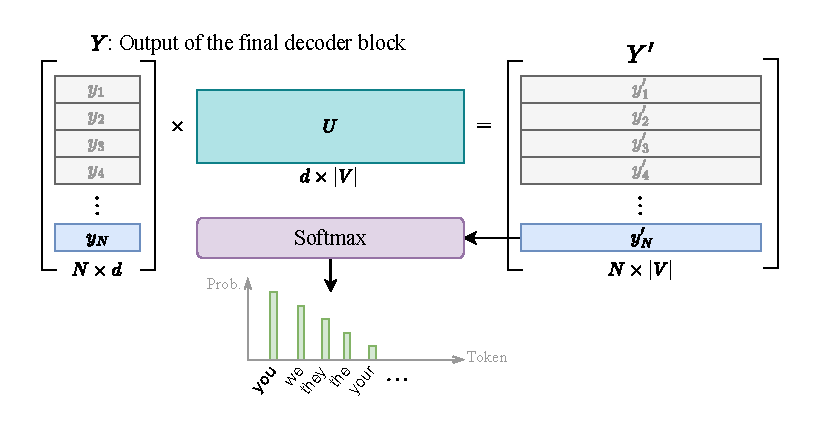
\includegraphics[width=1\linewidth]{fig/unembedding.pdf}
    \caption{Output unembedding layer.}
    \label{fig:unembedding}
\end{figure}

\section{Challenges and Conclusion}

Transformers face a few challenges, below are two prominent ones:

\begin{itemize}
    \item \textbf{Quadratic dependency on input length $d$}: As can be seen in Figure \ref{fig:QK^T}, this problem is inherent to the attention mechanism and prevents transformers from having large context window.
    \item \textbf{Interpretability}: Interpreting neural networks have always been a tough task, while transformer-specific interpretability \cite{mohebbi-etal-2024-transformer-interpret} raises even more challenges.
\end{itemize}

Eventually, this chapter is concluded with Figure \ref{fig:transformer}.


% \section{Conclusion}

% We have introduced all the ingredients in transformers. To sum up, we remark that a typical transformer consists of $L$ encoder and $L$ decoder blocks, where $L=6$ is chosen in \cite{vaswani2017attention}. This chapter is concluded with Figure \ref{fig:transformer}.

\begin{figure}
    \centering
    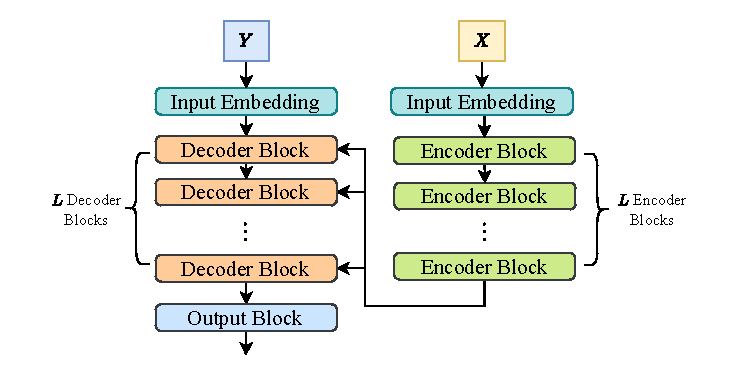
\includegraphics[width=1\linewidth]{fig/transformer.pdf}
    \caption{The transformer architecture, a closer look. Note that $L=6$ in the original paper \cite{vaswani2017attention}.}
    \label{fig:transformer}
\end{figure}